\section{Referencial teórico}
\label{sec:referencialTeorico}
% Os principais conceitos aos quais os trabalho está relacionado. Por exemplo, apresentar os conceitos de Aprendizado de Máquina e métodos relacionados.
% As principais técnicas e métodos nos quais o trabalho se apoia (referências)

Antes de tratar sobre as definições mais específicas que este trabalho vai utilizar, gostaria de trazer uma definição mais geral em que o problema está incluído. Podemos compreender Sistemas de Informação como sistemas, sejam eles manuais ou automatizados, inter-relacionados que atuam armazenando, processando e transmitindo dados que representam informações para as partes interessadas (\textit{stakeholders}). De forma mais geral, esses sistemas \enquote{\textit{atuam em conjunto para o cumprimento de uma tarefa ou um objetivo}} \cite{turban2009business}.

O grupo básico de operações de um Sistema de Informação é constituído pelas entradas, pelo processamento e pelas saídas (Figura \ref{fig:operacoesBasicaSistemas}). A entrada é o conjunto de dados que será usado pelo sistema, o processamento é composto pela transformações e combinações que os dados de entradas serão submetidos e, por fim, a saída é o produto obtido por meio do processamento dos dados de entrada. Em alguns casos, o sistema pode ser retroalimentado (\textit{feedback}), fazendo com que o resultado de saída seja manipulado como dados de entrada em uma nova execução. Nesse processo, também é comum que ocorra o armazenamento dos dados de entrada e de saída para serem utilizados posteriormente, como pode ser visto na Figura \ref{fig:operacoesBasicaSistemas}.

\begin{figure}[ht]
\centering
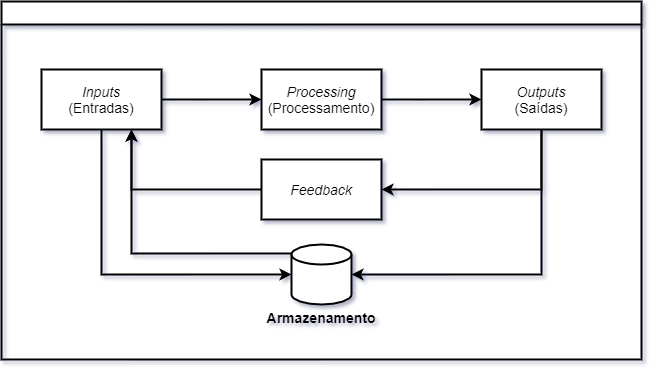
\includegraphics[width=1\textwidth]{imagens/operacoes-basicas-sistema-informacao.png}
\caption{Operações básicas de um Sistema de Informação.}
\label{fig:operacoesBasicaSistemas}
\end{figure}

Os dados que servem como entrada do sistema \enquote{\textit{são a menor parte de uma informação}} \cite{boscarioli2016mineracao} e podem ser definidos como conhecimento bruto ou fatos isolados. Nesse estado, podemos tê-los como não adequadamente tratados para fornecer gnose aos \textit{stakeholders}.

Por sua vez, a informação é a saída do sistema e descreve \enquote{\textit{qualquer conhecimento do mundo real... mas que apresenta algum significado ou valor para quem o detém}} \cite{boscarioli2016mineracao}. A informação é formada pelos dados de entrada do sistema após serem transformados, combinados \enquote{\textit{relacionados logicamente e organizados para atingir um resultado definido}} \cite{vida2021datawarehouse}, passando a fornecer conhecimento relevante para o processo de tomada de decisão.

Dessa maneira, temos os dados como matéria-prima do sistema e a informação como o produto. O nome de uma pessoa, uma data e um valor monetário são bons exemplos de dados, isolados eles não significam muito. No entanto, quando combinamos esses dados e atribuímos um significado ou contexto, como um depósito bancário, eles, os dados, passam a ter valor e se tornam informação.


Depois do processamento dos dados, e também antes, como já foi dito, os dados que compõem/comporão a informação precisam ser armazenados de maneira organizada. Para realizar essa organização é comum usar um banco de dados relacional (Figura \ref{fig:bancoDadosRelacional}), no qual \enquote{\textit{são conjuntos de dados organizados e relacionados entre si com registros sobre fatos, pessoas, empresas, coisas ou lugares.}} \cite{rezende2015obi}. Em vista disso, os bancos de dados são essenciais para os sistemas de informação.

\begin{figure}[ht]
\centering
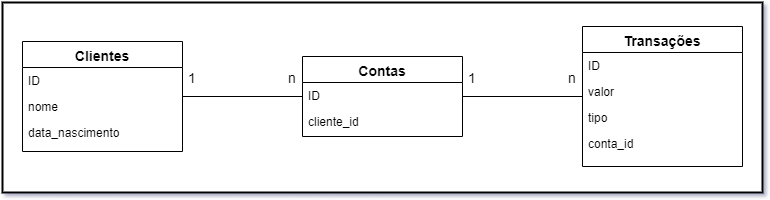
\includegraphics[width=1\textwidth]{imagens/banco-relacional.png}
\caption{Exemplo de descrição das tabelas de um banco de dados relacional}
\label{fig:bancoDadosRelacional}
\end{figure}

Vale destacar que um conjunto de dados composto por dados aleatórios não pode ser qualificado como um banco de dados, pois existem algumas características que devem ser atendidas para que seja classificado como tal.

\begin{itemize}
  \item Minimundo: O banco de dados deve representar uma parte do mundo real.
  \item Dados com significado: O banco de dados também tem que ser constituído por um conjunto lógico de dados que apresente algum significado.
  \item Dados com objetivo: Os dados que integram o banco necessitam ter ou cumprir um objetivo claro para o usuário ou aplicação, sendo prescindível o armazenamento dos dados que não contribuem com o propósito. \cite{vida2021datawarehouse}
\end{itemize} 

% TODO continuar falando sobre Data Warehouse https://integrada.minhabiblioteca.com.br/reader/books/9786556901916/pageid/20

\hfill

Ao longo das décadas, os computadores tiveram a sua capacidade de processamento e armazenamento aumentadas e juntamente com eles, houve um aumento da necessidade das empresas de investigar um grande volume de dados para nortear a sua tomada de decisão. Diante dessa necessidade, muitas abordagens foram criadas e \enquote{\textit{em 1988, o braço irlandês da IBM lançou o termo business data warehouse para valorizar os dados empresarias que estavam sendo armazenados. Em 1990, surgiu uma abordagem que ficou conhecida como data warehouses, sendo responsável pela cópia dos dados armazenados em arquivos e em banco de dados para outro local.}} \cite{vida2021datawarehouse}. Os dados que ficam armazenados nesse \enquote{novo} banco de dados (\textit{data warehouse}) são provindos de diversas base de dados oriunda das distintas áreas da empresa e serve para consolidar o conhecimento dessa pluralidade de base de dados.